\chapter{Pipeline benchmarking on \ac{NZ} data}
\label{chap:benchmark}

\section*{Summary}

A benchmark dataset was run through the programmes presented in chapters \ref{chap:pipeline} and \ref{chap:model} to showcase their performance. The experimental desgin attempted to capture a protein profile change reflecting a known biological process. Thus, a successful computational analysis of the dataset should also reflect the phenomenon. The results confirmed that the computational analysis successfully captured this response. It was concluded that the software can be used in future experiments where the biological phenomena underlying the data are not known.

\section{Introduction}

The protein ratios across conditions are not known in ordinary datasets In order to judge the resolving power of the mass spectrometry and shotgun proteomics workflows presented in this work, an in-house dataset attempting to capture an immunological response was generated. Therefore, even though true protein ratios were not known \textit{a priori}, the analysis should find proteins related to the immunological response to be significantly differentially abundant. 

Moreover, a function inference step from the estimated protein \ac{log2FC} values is required to arrive to biological interpretations like that. These kind of analysis is common to all omics (genomics, transcriptomics, ...) and can be completed with Gene Set Enrichment Analysis \ac{GSEA} and Pathway Analysis, among others.

\subsection{Goals}

\begin{enumerate}

\item Gauge the analytical power of the computational analyses explained in the previous chapters.

%\item Compare its results with the commercial software currently in use.

\item Propose a function inference analytical pipeline to complete the proteomics workflow.

\end{enumerate}


\section{Materials and Methods}

\subsection{Sample preparation}

THP-1 cells were grown in RPMI1640 (Sigma) supplemented with 10\% FBS (SeraLab) and 1\% pen/strep (Gibco). Stimulation of THP-1 cells was done in 48-well plates (Gibco) with 2x106 cells/well. Cells were exposed to 500 ng/mL LPS (E. coli O111:B4) (positive control condition, \textit{PC}) or nothing (negative control condition, \textit{NC}) for 48 hours in 37 degrees, 5\% \ce{{CO}_2}. After stimulation supernatants were collected and cell pellets were washed in PBS (Gibco). Both supernatants and pellets were frozen (-20 degrees). Only the pellet samples were considered for the analysis. EGWS, Esben Gjerløff Wedebye Schmidt.
 
\subsection{Mass Spectrometry analysis}

AEGI

\subsection{Computational analysis}

The resulting .RAW files were processed with the two different pipelines fully developed in the present work. (I) Compomics+MSqRob and (II) Compomics+BQ (Compomics and BayesQuant). The search settings were identical to those used in chapter \ref{chap:pipeline}, except for the proteome databases employed, which consisted of \textit{Homo sapiens} only. The validation filters, \ac{MBR}, MS1 Apex intensity, and MSqRob preprocessing parameters were also set to those used previously, for simplicity. The two pipelines used thus diverged only in the quantification engine, being identical in all previous steps.

In the Compomics+MSqRob pipeline, a protein was declared to be differentially abundant (\ac{DAP}) between the 2 conditions assayed if the result of the student\textquotesingle s-T test implemented in MSqRob returned a q-value less than 0.05. The criteria in the Compomics+BayesQuant pipeline was the absence of overlap between the \ac{ROPE} [-0.4, 0.4] and the 95\% \ac{HPDI}.


\subsection{Biological inference}

The gProfiler R package \cite{Boyd2010} was used to run automatic \ac{GSEA} and provide a biological interpretation of the results.

Pathways analysis was executed by calling the ComPath Webserver \cite{Domingo2018}. UniprotKB IDs were transformed to "Gene name" IDs, as required by the tool using the Retrieve/ID mapping tool from Uniprot. The KEGG \cite{Kanehisa2000} and Reactome \cite{Croft2014} databases were used as source.

Protein interactions were explored by querying the STRING database \cite{Szklarczyk2017} with the list of \ac{DAP}s produced by MSqRob.
 
\section{Results}

\subsection{Compomics+MSqRob}

Data on 6444 peptides, as collected in the peptide summary file from moFF, was passed to MSqRob, resulting in the quantification of 1433 proteins. A histogram of the \ac{log2FC} reveals that in most cases, not enough evidence was collected to declare the \ac{log2FC} different from 0 (see figure \ref{fig:compomics_rob} A). Remarkably, the distribution was shifted toward negative values, depicting that most of the proteins for which an non-null estimate was provided were more abundant in the \textit{PC} condition. A volcano plot (see figure \ref{fig:compomics_rob} B), reveals that the majority of the 49 protein groups passing the significance criteria ($qval < 0.05$), displayed an absolute value of the \ac{log2FC} less than 1. However, all were considered differentially abundant. The 32 protein groups composed by a single protein (single protein \ac{DAP}s) are shown in table \ref{tab:thp1_rob_results}.

% latex table generated in R 3.4.4 by xtable 1.8-2 package
% Sat Jul 21 16:02:33 2018
\begin{table}[!h]
\centering
\begin{tabular}{rllrr}
  \hline
 & Protein & Name & log2FC & qval \\ 
  \hline
  1 & P02792 & Ferritin light chain & 9.03E-01 & 2.32E-04 \\ 
  2 & Q04760 & Lactoylglutathione lyase & -7.24E-01 & 2.32E-04 \\ 
  3 & P13796 & Plastin-2 & -6.54E-01 & 2.32E-04 \\ 
  4 & P28066 & Proteasome subunit alpha type-5 & -6.88E-01 & 8.24E-04 \\ 
  5 & P09874 & Poly [ADP-ribose] polymerase 1 & -3.68E-01 & 2.48E-03 \\ 
  6 & P53396 & ATP-citrate synthase & -3.79E-01 & 3.25E-03 \\ 
  7 & P50552 & Vasodilator-stimulated phosphoprotein & -6.95E-01 & 1.43E-02 \\ 
  8 & P54577 & Tyrosine--tRNA ligase, cytoplasmic & -4.21E-01 & 2.71E-02 \\ 
  9 & Q15393 & Splicing factor 3B subunit 3 & -1.18E+00 & 2.88E-02 \\ 
  10 & P08567 & Pleckstrin & -1.26E+00 & 2.96E-02 \\ 
  11 & P50990 & T-complex protein 1 subunit theta & -3.60E-01 & 2.96E-02 \\ 
  12 & Q7RTV0 & PHD finger-like domain-containing protein 5A & -1.26E+00 & 2.96E-02 \\ 
  13 & O75083 & WD repeat-containing protein 1 & -6.55E-01 & 3.12E-02 \\ 
  14 & P17812 & CTP synthase 1 & -4.60E-01 & 3.12E-02 \\ 
  15 & Q14498 & RNA-binding protein 39 & -1.50E+00 & 3.29E-02 \\ 
  16 & P60903 & Protein S100-A10 & 1.13E+00 & 3.29E-02 \\ 
  17 & P26038 & Moesin & -3.91E-01 & 3.37E-02 \\ 
  18 & O75368 & SH3 domain-binding glutamic acid-rich-like p & -6.15E-01 & 3.37E-02 \\ 
  19 & Q8TEM1 & Nuclear pore membrane glycoprotein 210 & -8.24E-01 & 3.54E-02 \\ 
  20 & Q01518 & Adenylyl cyclase-associated protein 1 & -3.51E-01 & 3.54E-02 \\ 
  21 & Q08211 & ATP-dependent RNA helicase A & -4.19E-01 & 3.54E-02 \\ 
  22 & Q14566 & DNA replication licensing factor MCM6 & -4.33E-01 & 3.68E-02 \\ 
  23 & P30086 & Phosphatidylethanolamine-binding protein 1 & -6.31E-01 & 3.68E-02 \\ 
  24 & O43143 & RNA helicase DHX15 & -1.30E+00 & 3.80E-02 \\ 
  25 & O75691 & SMPC 20 homolog & -1.26E+00 & 3.80E-02 \\ 
  26 & P27797 & Calreticulin & -4.63E-01 & 3.80E-02 \\ 
  27 & P41218 & Myeloid cell nuclear differentiation antigen & -4.49E-01 & 3.80E-02 \\ 
  28 & Q15056 & Eukaryotic translation initiation factor 4H & -3.62E+00 & 3.98E-02 \\ 
  29 & P04406 & Glyceraldehyde-3-phosphate dehydrogenase & -1.90E+00 & 3.98E-02 \\ 
  30 & P00492 & Hypoxanthine-guanine phosphoribosyltransferase & -4.54E-01 & 4.12E-02 \\ 
  31 & P50440 & Glycine amidinotransferase, mitochondrial & -1.02E+00 & 4.50E-02 \\ 
  32 & P62857 & 40S ribosomal protein S28 & -5.50E-01 & 4.98E-02 \\ 
   \hline
\end{tabular}
\caption{THP-1 MSqRob results. 32 single-protein groups were found to be differentially abundant under significance criteria of q-value less than 0.05. The protein id, the gene name, the point estimate of its \ac{log2FC} and its significance is shown}
\label{tab:thp1_rob_results}
\end{table}


\begin{figure}[!h]
\begin{subfigure}{0.45\textwidth}
\centering
\caption*{A}
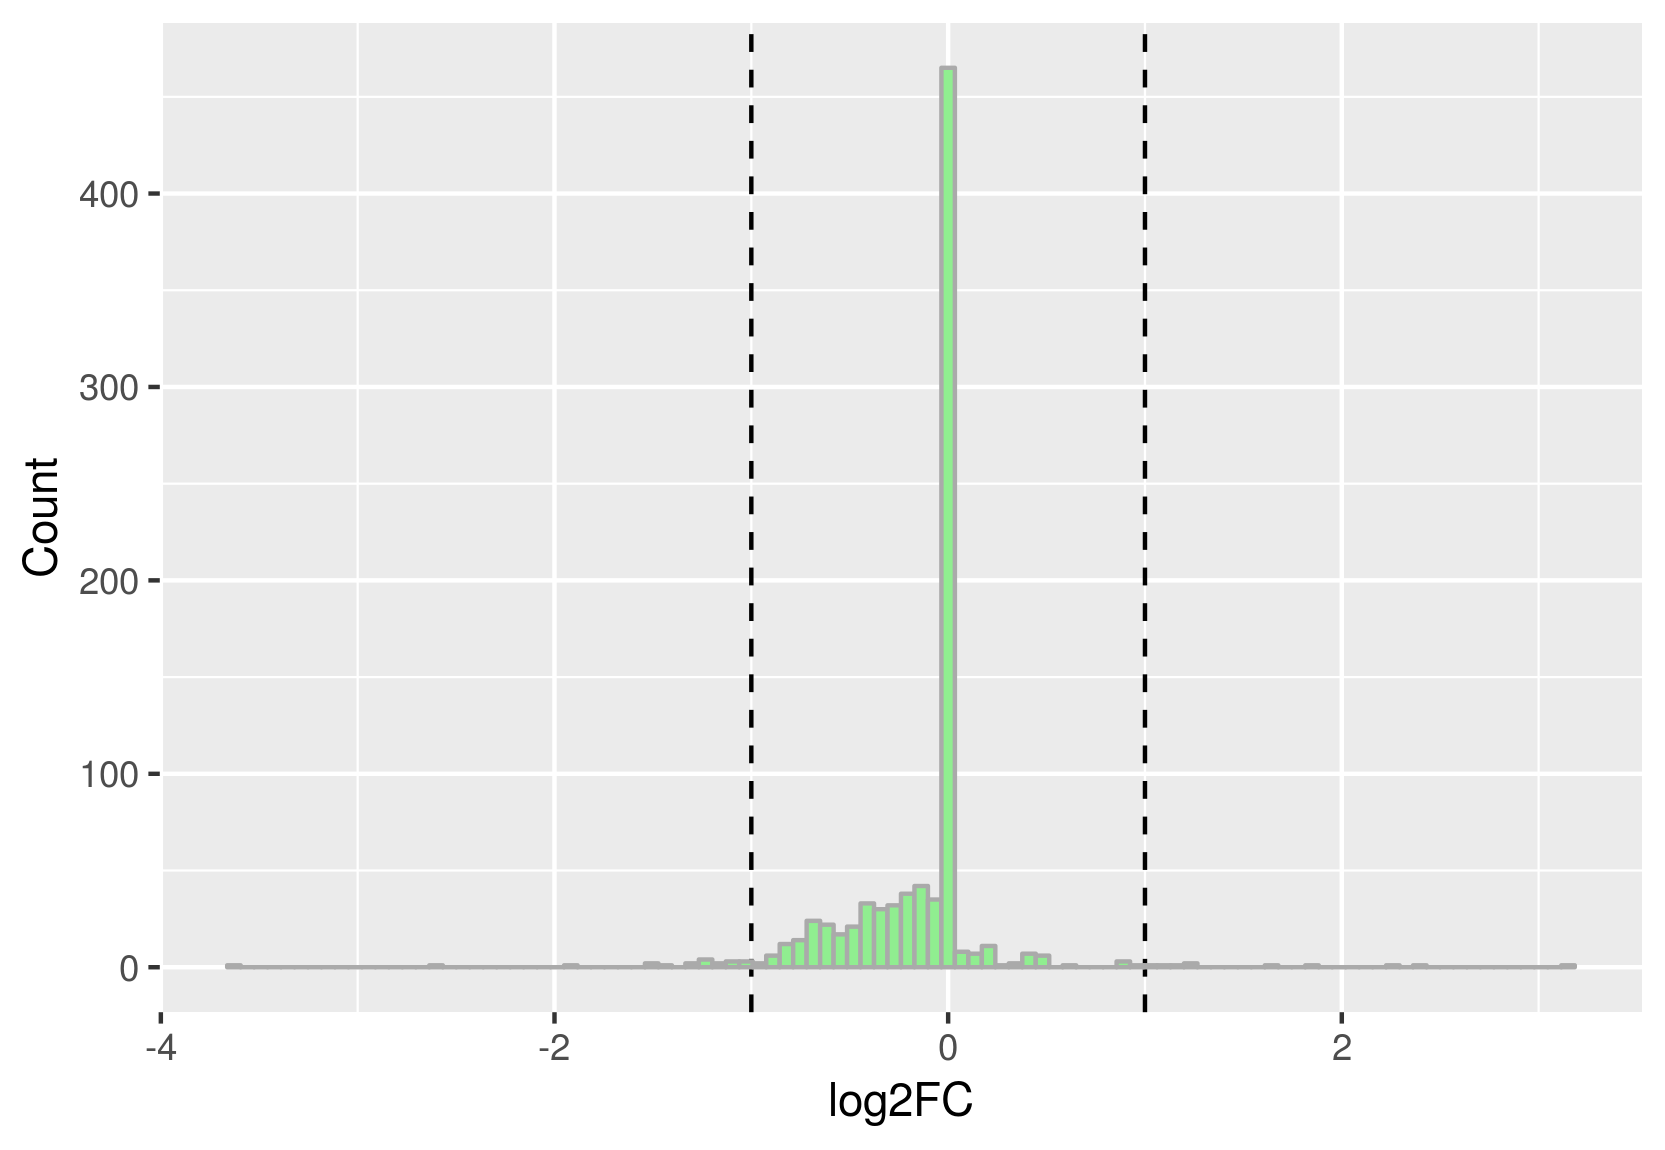
\includegraphics[width=.9\linewidth]{histogram_msqrob}
\end{subfigure}
\begin{subfigure}{0.45\textwidth}
\centering
\caption*{B}
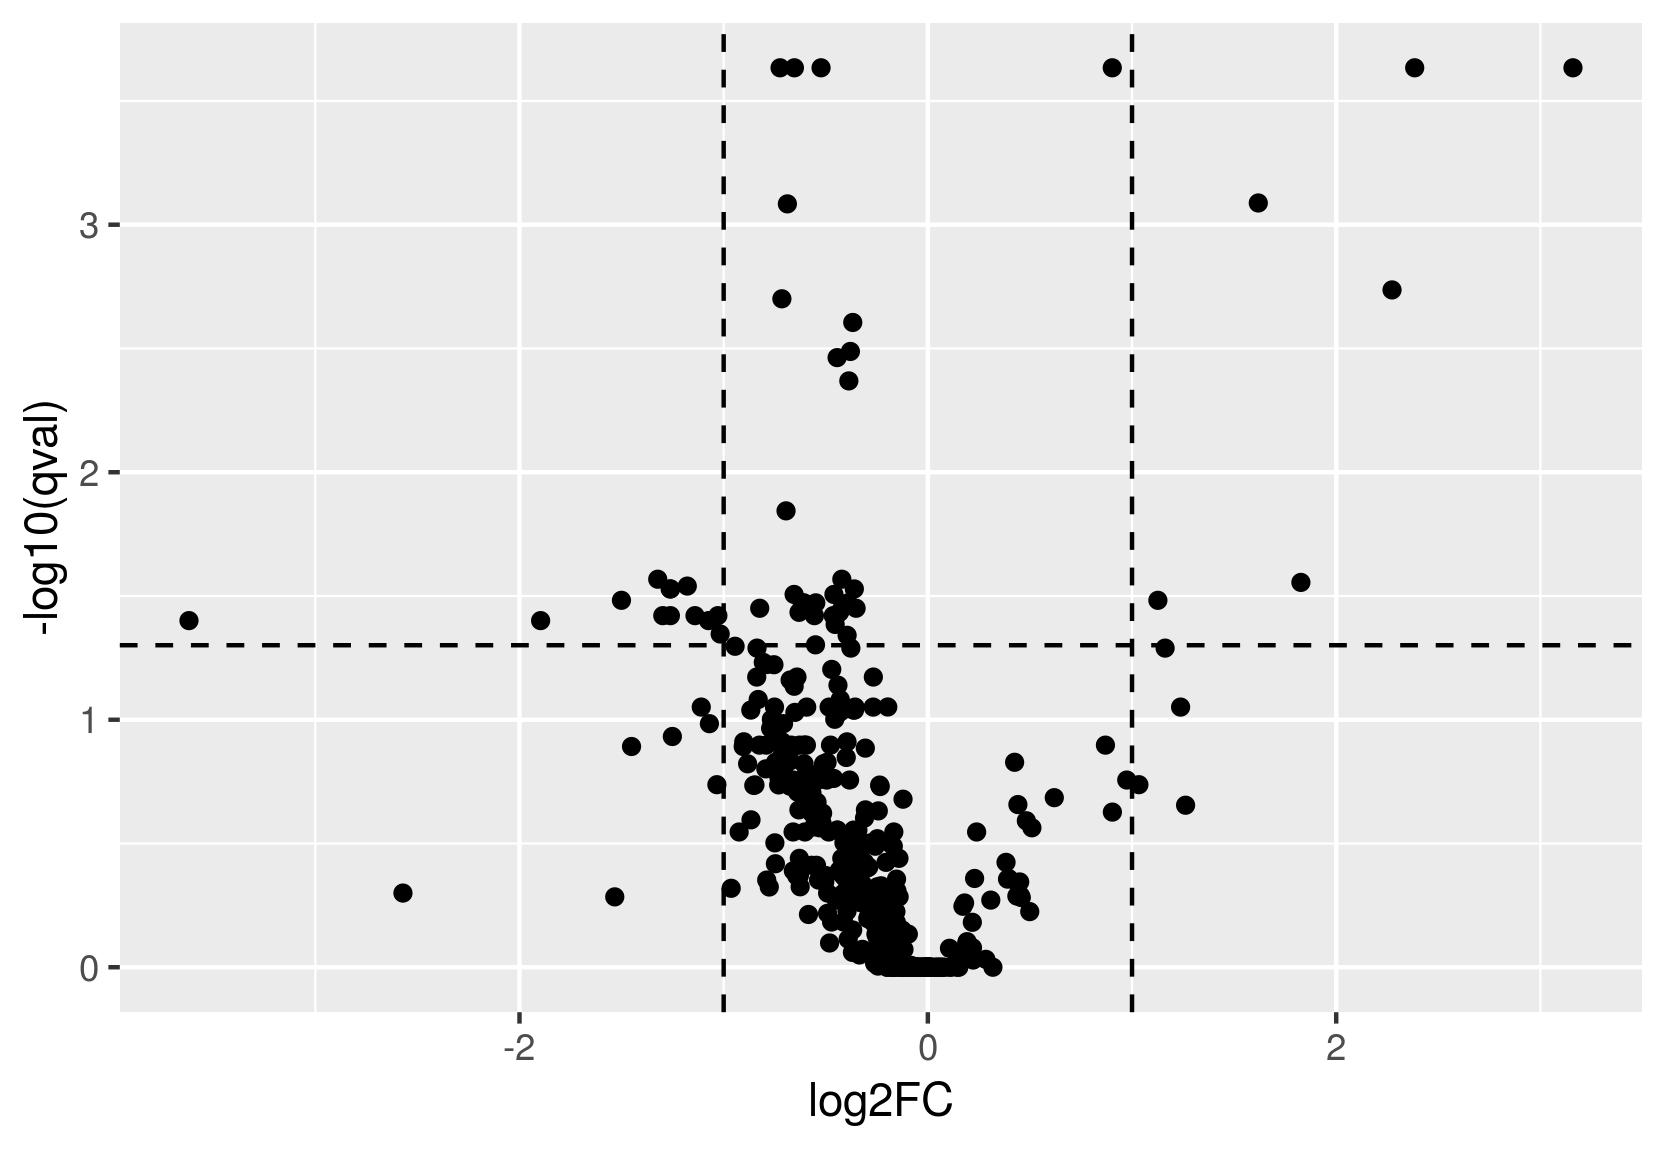
\includegraphics[width=.9\linewidth]{volcano_plot_msqrob}
\end{subfigure}
\caption[Compomics+MSqRob results on THP-1 dataset]{Compomics+MSqRob results. \textbf{A} Histogram of the estimated \ac{log2FC}. \textbf{B} Volcano plot, showing the point estimate of the \ac{log2FC} on the x axis, and the minus logarithm of the p-value on the y-axis.}
\label{fig:compomics_rob}
\end{figure}



\subsection{Compomics+BayesQuant}

After preprocessing and missing-data handling, a dataset of 1641 peptides was input to BayesQuant, and 269 proteins were quantified. A histogram of the mean of the inferred posterior distributions manifests the centrality of its distribution, with most values within the predefined \ac{ROPE} of [-0.4, 0.4]. In line with what was observed in the results above, the distribution was found to be skewed toward negative values (see figure \ref{fig:compomics_bq}A). Only four proteins were assigned a 95\% \ac{HPDI} not touching the \ac{ROPE} (see figure \ref{fig:compomics_bq}B and table \ref{tab:thp1_bq_results}). The distribution of the \ac{HPDI} width summarises the overall uncertainty in the estimation process. Most proteins had a very narrow HPDI, as shown in figure \ref{fig:compomics_bq}C. As expected, the width of the interval exhibited some degree of correlation with   the mean of the posterior, as shown in \ref{fig:compomics_bq}D.

% latex table generated in R 3.4.4 by xtable 1.8-2 package
% Sat Jul 21 18:02:39 2018
\begin{table}[!h]
\centering
\begin{tabular}{rlrrrr}
  \hline
 & Protein & log2FC & HPDI start & HPDI end & Peptides \\ 
  \hline
& O75475 & -0.61 & -0.80 & -0.43 & 2 \\ 
   & O15144 & -0.75 & -0.98 & -0.51 & 3 \\ 
   & P02792 & 0.50 & 0.41 & 0.58 & 4 \\ 
   & P04406 & -1.09 & -1.45 & -0.77 & 4 \\ 
   \hline
\end{tabular}
\caption{\ac{DAP} declared by the Compomics+BayesQuant pipeline.}
\label{tab:thp1_bq_results}
\end{table}


\begin{figure}[H]
\centering
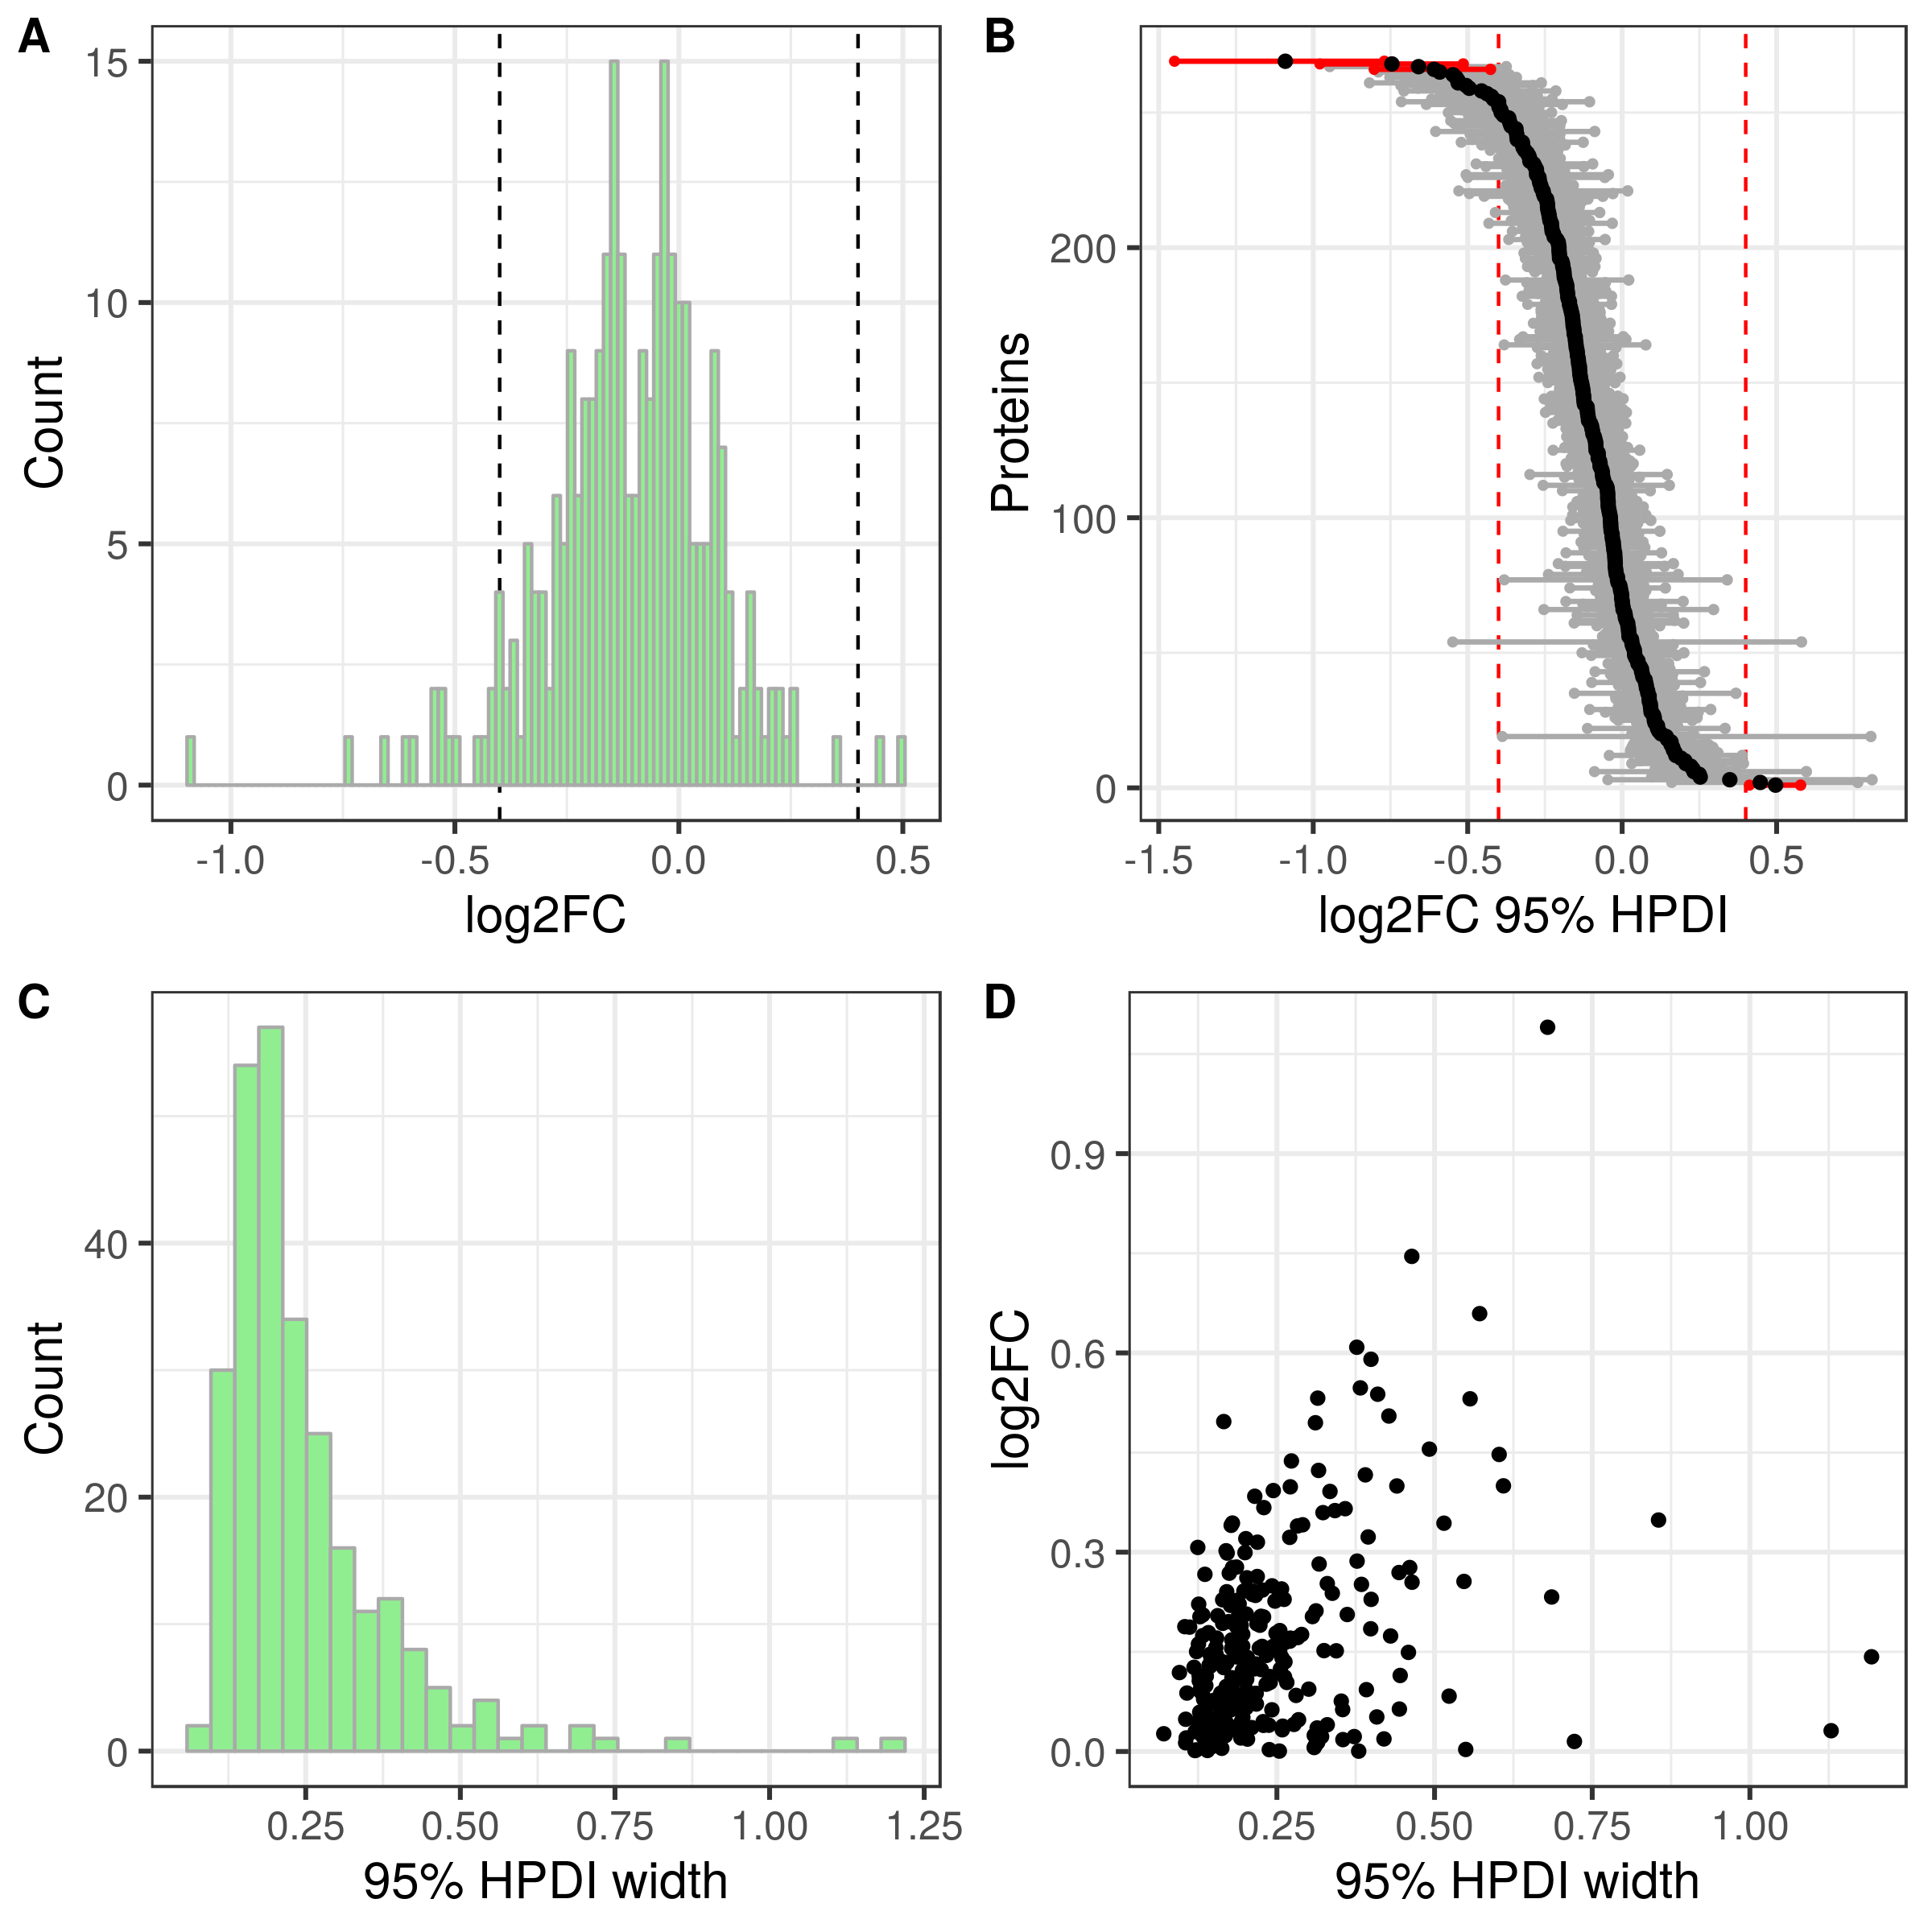
\includegraphics[width=\linewidth]{bq_comb_bq}
\caption[Compomics+BayesQuant results on the THP-1 dataset]{BayesQuant results. \textbf{A} Histogram of the mean of the posterior distributions. \textbf{B} Dumbbell plot, representing the 95\% \ac{HPDI} for all proteins. Black dots represent the mean, and intervals not overlapping the \ac{ROPE} are shown red. \textbf{C} Histogram of the 95\% \ac{HPDI} width. \textbf{D} Scatter plot of the 95\% \ac{HPDI} width and the  posterior \ac{log2FC} mean.}
\label{fig:compomics_bq}
\end{figure}


Given the scarcity of the results, it was decided to continue the analyses with MSqRob output only.

\subsection{Functional analysis}

A \ac{GSEA} performed on the list of 32 single-protein \ac{DAP}s produced by MSqRob (see table \ref{tab:thp1_rob_results}) illustrates the most overrepresented biological processes, cellular compartments and molecular functions, compared to the human background. The 20 most significant terms found in the dataset are displayed in table \ref{tab:gsea}.


% latex table generated in R 3.4.4 by xtable 1.8-2 package
% Sat Jul 21 19:00:27 2018
\small
\begin{table}[!h]
\centering
% latex table generated in R 3.4.4 by xtable 1.8-2 package
% Sun Jul 22 12:29:16 2018
\begin{tabular}{rllrrrl}
  \hline
 & Term ID & Term Name & Query & Term & Ov & P-value \\ 
  \hline
1 & GO:0070062 & extracellular exosome &  32 & 2774 &  19 & 1.17e-05 \\ 
  2 & GO:1903561 & extracellular vesicle &  32 & 2793 &  19 & 1.31e-05 \\ 
  3 & GO:0043230 & extracellular organelle &  32 & 2795 &  19 & 1.33e-05 \\ 
  4 & GO:0005615 & extracellular space &  32 & 3958 &  20 & 6.76e-04 \\ 
  5 & GO:0035578 & azurophil granule lumen &  32 &  90 &   5 & 8.87e-04 \\ 
  6 & GO:0044421 & extracellular region part &  32 & 4119 &  20 & 1.34e-03 \\ 
  7 & GO:0002376 & immune system process &  32 & 2949 &  17 & 1.74e-03 \\ 
  8 & GO:0060205 & cytoplasmic vesicle lumen &  32 & 335 &   7 & 2.54e-03 \\ 
  9 & GO:0031983 & vesicle lumen &  32 & 336 &   7 & 2.59e-03 \\ 
  10 & GO:0005576 & extracellular region &  32 & 4925 &  21 & 4.95e-03 \\ 
  11 & GO:0003723 & RNA binding &  32 & 1787 &  13 & 5.50e-03 \\ 
  12 & GO:0065003 & protein-containing complex assembly &  32 & 1803 &  13 & 6.08e-03 \\ 
  13 & GO:0003725 & double-stranded RNA binding &  32 &  65 &   4 & 9.71e-03 \\ 
  14 & GO:0005766 & primary lysosome &  32 & 153 &   5 & 1.23e-02 \\ 
  15 & GO:0042582 & azurophil granule &  32 & 153 &   5 & 1.23e-02 \\ 
  16 & HPA:006020\_13 & caudate; neuronal cells &  14 & 311 &   5 & 1.35e-02 \\ 
  17 & GO:0031982 & vesicle &  32 & 4271 &  19 & 1.38e-02 \\ 
  18 & GO:1990904 & ribonucleoprotein complex &  32 & 836 &   9 & 1.44e-02 \\ 
  19 & GO:0001775 & cell activation &  32 & 1359 &  11 & 1.60e-02 \\ 
  20 & HPA:022020\_13 & hippocampus; neuronal cells &  14 & 331 &   5 & 1.81e-02 \\ 
   \hline
\end{tabular}

%\begin{tabular}{rllllll}
%  \hline
% & Term ID & Term Name & Query & Term & Ov & P-value \\ 
%  \hline
%1 & GO:0070062 & extracellular exosome &  32 & 2774 &  19 & 1.17e-05 \\ 
%  2 & GO:1903561 & extracellular vesicle &  32 & 2793 &  19 & 1.31e-05 \\ 
%  3 & GO:0043230 & extracellular organelle &  32 & 2795 &  19 & 1.33e-05 \\ 
%  4 & GO:0005615 & extracellular space &  32 & 3958 &  20 & 6.76e-04 \\ 
%  5 & GO:0035578 & azurophil granule lumen &  32 &  90 &   5 & 8.87e-04 \\ 
%  6 & GO:0044421 & extracellular region part &  32 & 4119 &  20 & 1.34e-03 \\ 
%  7 & GO:0002376 & immune system process &  32 & 2949 &  17 & 1.74e-03 \\ 
%  8 & GO:0060205 & cytoplasmic vesicle lumen &  32 & 335 &   7 & 2.54e-03 \\ 
%  9 & GO:0031983 & vesicle lumen &  32 & 336 &   7 & 2.59e-03 \\ 
%  10 & GO:0005576 & extracellular region &  32 & 4925 &  21 & 4.95e-03 \\ 
%  11 & GO:0003723 & RNA binding &  32 & 1787 &  13 & 5.50e-03 \\ 
%  12 & GO:0065003 & Complex assembly &  32 & 1803 &  13 & 6.08e-03 \\ 
%  13 & GO:0003725 & DS RNA binding &  32 &  65 &   4 & 9.71e-03 \\ 
%  14 & GO:0005766 & primary lysosome &  32 & 153 &   5 & 1.23e-02 \\ 
%  15 & GO:0042582 & azurophil granule &  32 & 153 &   5 & 1.23e-02 \\ 
%  16 & HPA:006020\_13 & caudate; neuronal cells &  14 & 311 &   5 & 1.35e-02 \\ 
%  17 & GO:0031982 & vesicle &  32 & 4271 &  19 & 1.38e-02 \\ 
%  18 & GO:1990904 & ribonucleoprotein complex &  32 & 836 &   9 & 1.44e-02 \\ 
%  19 & GO:0001775 & cell activation &  32 & 1359 &  11 & 1.60e-02 \\ 
%  20 & HPA:022020\_13 & hippocampus; neuronal cells &  14 & 331 &   5 & 1.81e-02 \\ 
%   \hline
%\end{tabular}
\caption{\ac{GSEA} results. The 20 most significant terms are displayed. The columns \textit{Query}, \textit{Term} and \textit{Ov} indicate the size of the query, the number of proteins under the term, and the overlap between them. The size of the query differs in the GO and HPA terms repositories due to nomenclature mismatches.}
\label{tab:gsea}
\end{table}
\normalsize

On the one hand, nine terms (1, 2, 3, 4, 6, 8, 9, 10 and 17) were cell compartment terms associated with cellular secretion and the extracelullar space. On the other hand, five terms (5, 7, 14, 15, 19) were related to the immunological response. The remaining terms were connected to RNA functions and the nervous system.

\subsection{Pathway analysis}

The UniprotKB to Gene name mapping of the whole set of \ac{DAP}s (including multiprotein groups) returned by MSqRob returned a list of 51 entities. The list was supplied to the ComPath Pathway Enrichment tool to highlight which cellular pathways were overrepresented compared to the human background. In agreement with the \ac{GSEA} results, a handful of pathways linked to the immune response were found to be significantly enriched: (I) Immune System, (II) Innate Immune System, (III) Necroptosis (IV) Programmed Cell Death, (V) Regulation of Apoptosis, (VI) Leukocyte transedothelial migration. Moreover, the finding of several RNA related pathways exposes the presence of potential cell reprogramming, essential in any change in protein profile.

% latex table generated in R 3.4.4 by xtable 1.8-2 package
% Sat Jul 21 19:49:28 2018
\begin{table}[ht]
\centering
\begin{tabular}{rllrrl}
  \hline
 & Pathway & q-val & Ov & Size & DB \\ 
  \hline
1 & Neutrophil degranulation & 0.00e+00 &   9 & 479 & reactome \\ 
  2 & Immune System & 0.00e+00 &  15 & 2050 & reactome \\ 
  3 & Innate Immune System & 0.00e+00 &  10 & 1109 & reactome \\ 
  4 & Metabolism of RNA & 0.00e+00 &  10 & 666 & reactome \\ 
  5 & Processing of Pre-mRNA & 2.00e-04 &   5 & 240 & reactome \\ 
  6 & mRNA Splicing & 1.10e-03 &   4 & 180 & reactome \\ 
  7 & mRNA Splicing & 1.20e-03 &   4 & 188 & reactome \\ 
  8 & Metabolic pathways & 1.60e-03 &   8 & 1282 & kegg \\ 
  9 & Carbon metabolism & 2.90e-03 &   3 & 116 & kegg \\ 
  10 & Spliceosome & 4.00e-03 &   3 & 134 & kegg \\ 
  11 & Pentose phosphate pathway & 4.20e-03 &   2 &  30 & kegg \\ 
  12 & Base excision repair & 4.90e-03 &   2 &  33 & kegg \\ 
  13 & Ribosome & 5.30e-03 &   3 & 153 & kegg \\ 
  14 & Necroptosis & 6.10e-03 &   3 & 162 & kegg \\ 
  15 & Apoptosis & 6.60e-03 &   3 & 168 & reactome \\ 
  16 & Programmed Cell Death & 6.90e-03 &   3 & 171 & reactome \\ 
  17 & Regulation of Apoptosis & 1.08e-02 &   2 &  53 & reactome \\ 
  18 & Aminoacyl-tRNA biosynthesis & 1.55e-02 &   2 &  66 & kegg \\ 
  19 & Glycolysis / Gluconeogenesis & 1.59e-02 &   2 &  68 & kegg \\ 
  20 & Leukocyte transendothelial migration & 2.96e-02 &   2 & 112 & kegg \\ 
   \hline
\end{tabular}
\caption{Pathway Enrichment results. The 10 most significant pathways found in Reactome and Kegg are shown arranged by decreasing significance. }
\label{tab:pathway_enrichment}
\end{table}

\subsection{Protein interaction analysis}

The same list supplied to ComPath was searched in the STRING database \cite{Szklarczyk2017} to screen for protein-protein interactions in the list. The database returns a protein association network (see figure \ref{fig:STRING}), that helps interpreting the information contained in gene sets. 49/51 terms were mapped to the resource and 15 of them were found to be included in the "immune system process" set, placing the biological process as the third most enriched with an FDR of 0.0387. 27 genes belonged to the "cellular nitrogen compound metabolic process" (FDR 0.0128).

\begin{figure}[!h]
\centering
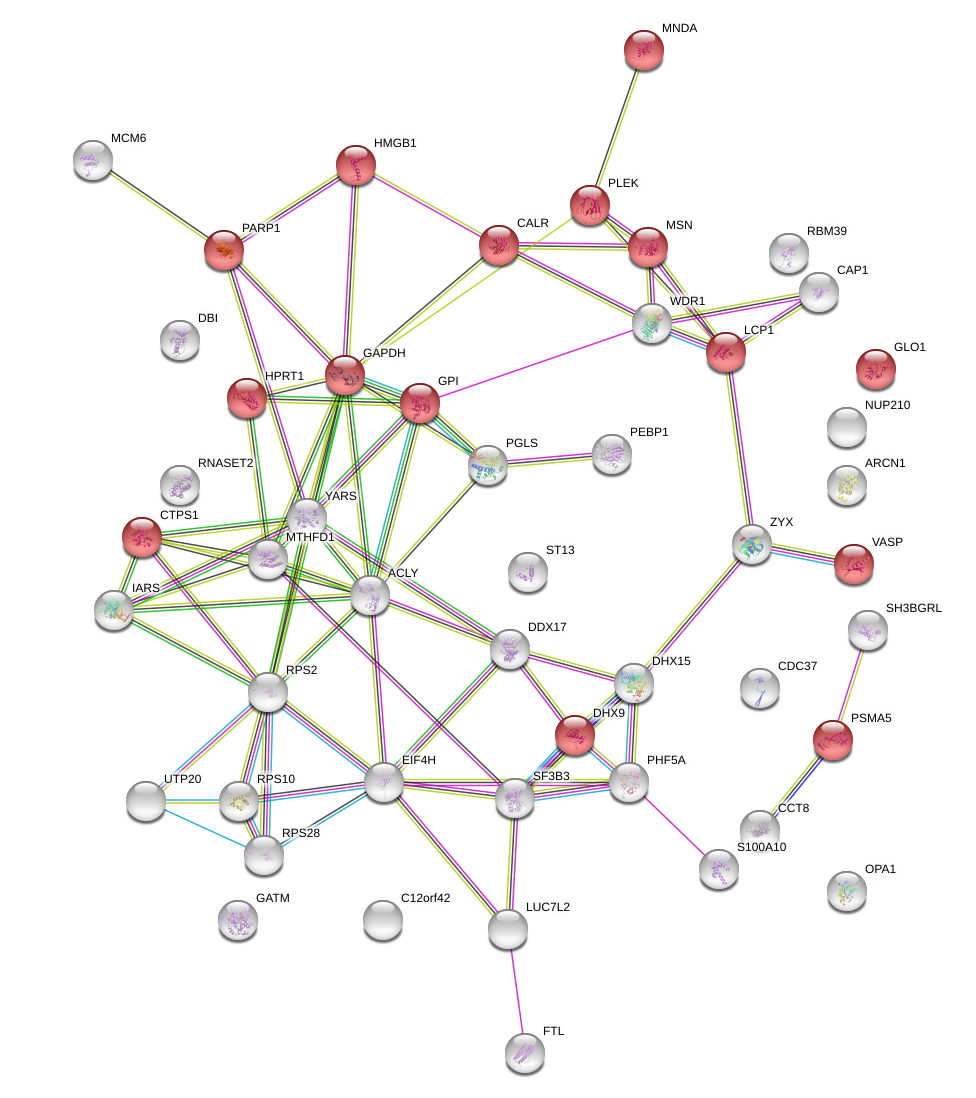
\includegraphics[width=\linewidth]{string_normal_image}
\caption[Protein interaction network]{STRING interaction network. Every node represents a protein in the list, and an edge between any pair represents evidence for some kind of association or interaction between them. Evidence is either experimentally determined or predicted using diverse methods. Red colored nodes are included in the "immune system process" set.}
\label{fig:STRING}
\end{figure}





\section{Discussion}

\subsection{Increasing the experiment data-throughput}

6 samples organized in two different treatments of 3 biological replicates without sample prefractionation each were analyzed. The resulting data throughput allowed for the performance of biological inference, as it successfully captured the undergoing biological processes. Nevertheless, a more in-depth results report would have been possible with (I) sample prefractionation, which improves peptide separation and allows for the collection and identification of more spectra \cite{Righetti2005}, and (II) the inclusion of technical replicates to differentiate the biological variability from experimental noise.

\subsection{Missing data handling}

One of the most frequent issues found when analyzing proteomics datasets is the handling of missing values \cite{Lazar2016}. The presence of missing data in many of the rows in the input moFF file led to the dropping of 4803 out of 6443 peptides, producing a peptide dataset of only 1641 data points that accounted for 350 protein groups. Thanks to the missing data handling implemented in MSqRob quantified 1433 proteins, enough to continue the analysis (see table \ref{tab:balance}). The fact that the number of observed groups was 2787 implies that the management of missing values could be improved in both tools, and particularly in BayesQuant.

\begin{table}[!h]
\centering
\begin{tabular}{|c|c|c|}
\hline 
Tool & Peptides & Proteins \\ 
\hline 
MSqRob & 6444 & 1433 \\ 
\hline 
BayesQuant & 1641 & 350 \\ 
\hline 
\end{tabular} 
\caption{Peptide input and quantified proteins for each tool in the THP1 dataset.}
\label{tab:balance}
\end{table}

Three different types of missing values have been defined \cite{Wei2018}:

\begin{enumerate}

\item Missing Completely At Random (MCAR): Unpredictable, caused by random errors in the data acquistion step and affecting the whole dataset.

\item Missing At Random (MAR): Caused by other observed variables. Citing \cite{Wei2018}: \textit{ Inaccurate peak detection and deconvolution of co-eluting compounds can be called MAR}.

\item Missing Not At Random (\ac{MNAR}): Caused by signals under the limit of detection (\ac{LOD}) of the spectrometer.

\end{enumerate}

While all three are relevant, \ac{MNAR} is particularly important because it introduces a bias in the dataset, where proteins are more likely to be quantified if their abundance is high enough in all samples for their peptide signals to be above the \ac{LOD}. Thus, proteins exhibiting abundances below the \ac{LOD} due to the experimental treatment are bound to generate peptide data featuring missing values that, if not handled properly, are discarded. Subsequently, \ac{DAP}s or in general proteins with variant abundance become less likely to be quantified, difficulting the extraction of protein sets.

Missing data should be imputed at the peptide level. The implementation of a module performing this task prior to quantification would  improve the accuracy and throughput of the quantification process. Several approaches have been proposed, some within a probabilistic framework \cite{Lazar2016}. For example, in cases of clear \ac{MNAR}, imputation could be based on an inferred global \ac{LOD}, so that missing values are replaced with it. Work on this line could potentially boost the performance of BayesQuant.


\subsection{Applicability for Novozymes data}

\ac{NZ} data is frequently confidential and cannot be uploaded to public servers like STRING. However, many of the databases consulted in this work can be built locally, thus removing the need of data leaving the company\textquotesingle s facilities.



\section{Conclusion}
The results presented in this work demonstrated the usability of the tools presented in the previous chapters in an actual \ac{NZ} setting. Moreover, a walk-through over the functional analyses that can be performed with this output clearly showed they can be used to perform computational analyses and biological inference on protein samples with open-source software with no cost for the company. However, the absence of proper missng data handling developed into the inability to quantify hundreds of proteins, signaling what are the next steps to improve the tools.